\chapter{Benchmarks: method, results, and how to read them}\label{ch:bench}

\begin{warn}[Sandbox numbers, not cluster numbers]
Every number in this chapter was measured in the sandbox where the code was written: \sbxCpu, 2 visible cores, a virtual machine, \sbxCompiler, run on \sbxDate. They illustrate what each experiment looks like and what conclusions it supports. They are \textbf{not} bwUniCluster results and must never be quoted as such. Chapter~\ref{ch:cluster} gives the scripts that produce the same tables and figures on the cluster; those numbers are yours to measure. If you have older cluster results for this project from an earlier version of the code, they came from different code and are not comparable with anything here.
\end{warn}

\section{Method}

The benchmark program (\file{apps/simdip\_bench.cpp}) uses one method for every configuration:
\begin{enumerate}
\item Allocate and fill the images \emph{before} timing, so that page-fault cost is not measured.
\item Two warm-up calls (cache, branch predictors, OpenMP thread pool), then one call to estimate the duration and choose an iteration count so that one sample lasts at least \code{--min-ms} (20 ms by default).
\item Take \code{--reps} samples (7 to 9), each the average time per call over that many iterations. Report the \textbf{median}, plus minimum and maximum. The median is robust against an occasional disturbance by another job on a shared machine; the minimum is the best case.
\item Throughput: output pixels per second (Mpixel/s). \emph{GB/s} is the minimum traffic (each source byte read once, each destination byte written once) divided by time, a lower bound of what the memory system moved. GFLOP/s for convolution counts $2k^2$ per pixel.
\item The program prints the CPU model, compiler, whether the build is optimised, and \code{OMP\_PROC\_BIND}/\code{OMP\_PLACES}, so a pasted result carries its own provenance. Slurm jobs additionally write \file{meta.txt}.
\end{enumerate}

\textbf{Fairness of the comparison.} The three implementations run the same image, the same kernel and the same method. ``Scalar'' is compiled with the auto-vectorizer switched off, ``autovec'' with it on, both with FMA contraction off, so that the only difference between them is the compiler's vectorization. The hand-written AVX2 path is compiled separately with \code{-mavx2 -mfma}. The plain \code{-O3} build targets baseline x86-64 (SSE2), which is what ``autovec'' means here; a build with \code{-march=native} lets the compiler use AVX2/AVX-512 and is available as an option in the cluster script (\code{NATIVE=1}). Quote ``autovec'' as ``GCC \code{-O3} auto-vectorization, SSE2 baseline''.

\section{Main results}

\begin{center}
\small
\begin{tabularx}{\textwidth}{@{}l r X X X X@{}}
\toprule
2048$\times$2048 & scalar (ms) & autovec (ms) & AVX2 (ms) & scalar, 2 threads & AVX2, 2 threads\\
\midrule
\inputrows{snippets/tab_e1}
\end{tabularx}
\captionof{table}{Median time per call, with speedup over single-thread scalar in brackets (sandbox, 2 cores).}
\end{center}

\begin{center}
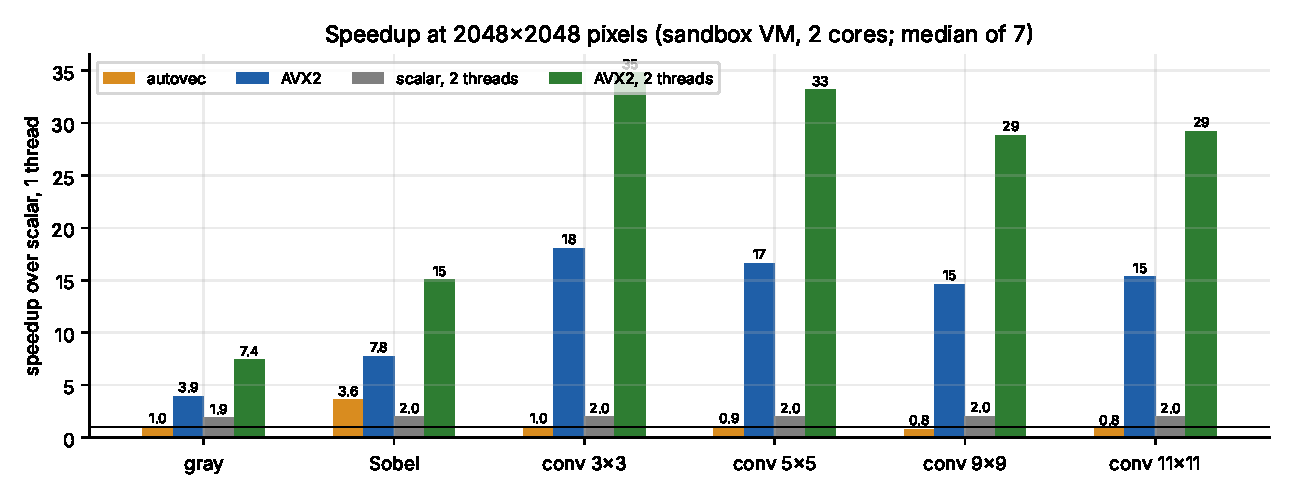
\includegraphics[width=0.95\textwidth]{figures/f_speedup.pdf}
\captionof{figure}{Speedups over single-thread scalar at 2048$\times$2048.}
\end{center}

What these data say, each point tied to a number:
\begin{itemize}
\item \textbf{AVX2 is the dominant factor.} On one thread it is \spGrayAvx$\times$ faster than scalar for gray, \spSobelAvx$\times$ for Sobel and \spConvNineAvx$\times$ (9$\times$9) to \spConvThreeAvx$\times$ (3$\times$3) for convolution; the convolution figure is lowest for the larger kernels because it is the scalar baseline that benefits from nothing and the vector kernel that approaches its FMA ceiling. The speedup of convolution is much larger than the 8 lanes of a float vector because the scalar code needs separate multiply, add, load and index instructions per tap (and cannot be auto-vectorized, see below), whereas AVX2 retires one fused multiply-add on eight pixels per instruction.
\item \textbf{GCC's auto-vectorizer helps Sobel, not gray or convolution.} It reaches \spSobelAutovec$\times$ on Sobel, but \spGrayAutovec$\times$ on gray (the vectorization report marks the loop as failed; the interleaved 3-byte RGB access is the likely cause but the report does not say so) and \spConvThreeAutovec$\times$ ($3\times3$) down to \spConvElevenAutovec$\times$ ($11\times11$) on convolution, i.e.\ no gain and for the larger kernels slightly slower than scalar (the report names the loop-nest structure, Chapter~\ref{ch:scalar}). Chapter~\ref{ch:scalar} shows the report and which of these statements the compiler makes itself and which are interpretation.
\item \textbf{OpenMP scales as the hardware allows.} With two threads scalar code gives about 2$\times$ (\spGrayScalarTwo, \spSobelScalarTwo, \spConvThreeScalarTwo), and AVX2 with two threads \spGrayAvxTwo$\times$, \spSobelAvxTwo$\times$ and \spConvThreeAvxTwo$\times$ over single-thread scalar: the two factors multiply. At 4096$\times$4096 two threads give \scaleGrayAvxFourK$\times$ (gray), \scaleSobelAvxFourK$\times$ (Sobel) and \scaleConvAvxFourK$\times$ (convolution 9$\times$9) over one thread, i.e.\ close to perfect scaling \emph{on this machine}, because two threads do not saturate its memory (Chapter~\ref{ch:cache}). That does not carry over to 32 or 64 cores: gray and Sobel will flatten once the memory system is saturated, convolution much later. The scaling script exists to measure exactly this.
\end{itemize}

\begin{center}
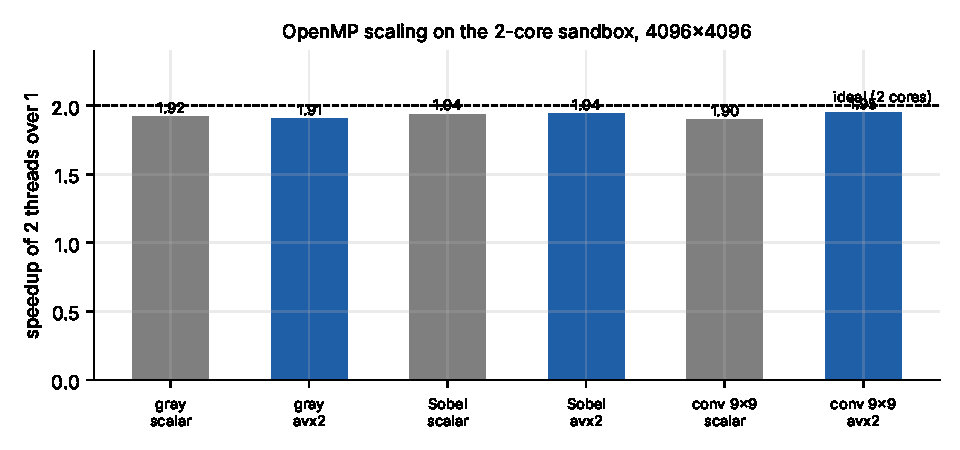
\includegraphics[width=0.8\textwidth]{figures/f_threads.pdf}
\captionof{figure}{Two threads versus one at 4096$\times$4096.}
\end{center}

\section{Convolution: kernel size and the ablations}

\begin{center}
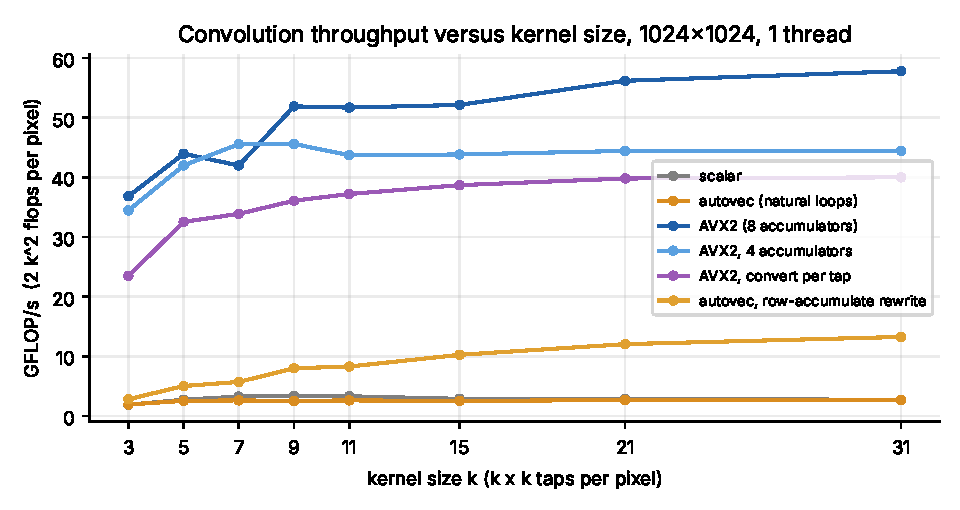
\includegraphics[width=0.85\textwidth]{figures/f_conv_ksize.pdf}
\captionof{figure}{Convolution rate versus kernel size (1024$\times$1024, one thread).}
\end{center}

\begin{center}
\small
\begin{tabular}{@{}lrrr@{}}
\toprule
GFLOP/s, 1024$^2$, 1 thread & $k=3$ & $k=9$ & $k=31$\\
\midrule
\inputrows{snippets/tab_ablation}
\end{tabular}
\end{center}

\begin{itemize}
\item \textbf{Throughput rises with $k$ and then flattens at \gfAvxMax\,GFLOP/s}, about \fracOfNominalPeak\,\% of the nominal peak of one core (Chapter~\ref{ch:cache}). For $k=3$ the fixed per-row costs (converting a row to float, writing the output) are a larger share of the work (\gfAvxThree\,GFLOP/s); for large kernels the FMA units dominate. Scalar stays below \gfScalarMax\,GFLOP/s throughout.
\item \textbf{Eight accumulators beat four}: \ratioAccFourNine$\times$ at $k=9$ and up to \ratioAccFourMax$\times$ for larger kernels: with fewer independent FMA chains the 4-cycle FMA latency is no longer hidden (Chapter~\ref{ch:conv}).
\item \textbf{Converting per tap costs} a factor \ratioPerTapNine\ at $k=9$: converting each byte to float for every tap rather than once per row spends instructions that compete with the FMAs.
\item \textbf{Helping the compiler} (the row-accumulate rewrite, bit-identical to scalar) gives \gfRowAccNine\,GFLOP/s at $k=9$, \ratioRowAccToNatural$\times$ the natural-loop autovec but still \ratioRowAccToAvx$\times$ below the hand-written kernel. The compiler got a long way once the loop was restructured; the remaining gap is plausibly the register blocking of the hand-written kernel (eight accumulators held in registers for a whole block of pixels across all $k^2$ taps); the experiment shows the gap, not its cause, and a look at the generated assembly would be needed to be sure.
\end{itemize}
Those four statements are the answer to ``why not just let the compiler do it?'': it is a measured, quantified answer.

\section{Comparison with OpenCV}

\begin{center}
\small
\begin{tabular}{@{}lrrr@{}}
\toprule
2048$\times$2048, 1 thread & OpenCV (ms) & this library, AVX2 (ms) & OpenCV / ours\\
\midrule
\inputrows{snippets/tab_opencv}
\end{tabular}
\end{center}

This comparison is useful for orientation and dangerous as a claim. The caveats are part of the result:
\begin{itemize}
\item OpenCV was installed with \code{pip} in the sandbox (version 5.0.0, 1 thread, ``optimized: True''); its build and CPU dispatch (which instruction sets it chose on this VM) were not inspected.
\item Gray: OpenCV uses 14-bit coefficients, so its output differs from ours by up to one level on 7.4\,\% of pixels: it does more precise work.
\item Sobel: our function is one fused pass producing $\min(255,|G_x|+|G_y|)$; the OpenCV figure is two \code{Sobel} calls in 16-bit, absolute values, a saturating add, i.e.\ a \emph{pipeline} of several full-image passes and temporary images. Part of the \ocvSobel$\times$ is fusion, not SIMD quality.
\item Convolution: \code{filter2D} handles border modes, depths and arbitrary kernels and allocates its output; it agrees with ours to within one level on every tested kernel (identical for $3\times3$).
\item Python call overhead is included in the OpenCV time; at 2048$^2$ it is negligible (microseconds against milliseconds).
\end{itemize}
The defensible sentence is: ``On this machine my AVX2 kernels run \ocvGray$\times$ to \ocvConvNine$\times$ faster than the corresponding OpenCV calls for gray and convolution and about \ocvSobel$\times$ for the Sobel pipeline, where most of that comes from doing it in one pass; OpenCV supports far more and I do not claim to replace it.'' The indefensible sentence is ``faster than OpenCV''.

\section{Repeatability: how big is a ``real'' difference?}

Two different spreads were measured, and the second one is the larger and the more instructive.
\begin{itemize}
\item \textbf{Within one job (E6).} The same 24 measurements repeated three times in a row differ by up to \repSpreadOne\,\% between repetitions for single-thread runs and up to \repSpreadTwo\,\% for two-thread runs (the host is shared; with two threads on a 2-vCPU guest any background activity lands on a thread of the benchmark).
\item \textbf{Between two passes minutes apart.} The main experiment (E1) was run twice with the identical command; the first pass is kept in \file{results/sandbox\_example/firstrun/}. For image sizes of 1024 and above, the median difference between the two passes was \betweenScalarMed\,\% for the scalar implementation (largest: \betweenScalarMax\,\%), \betweenAutovecMed\,\% for autovec (largest \betweenAutovecMax\,\%) and only \betweenAvxMed\,\% for AVX2 (largest \betweenAvxMax\,\%). The scalar convolution was the main culprit: in the first pass it ran slower by up to about 40\,\% on many configurations, for a reason I cannot identify from inside a virtual machine (other tenants on the host, a different clock state, or both). All numbers in this chapter come from the second pass, and the other experiments were repeated after it for consistency.
\end{itemize}
Consequences:
\begin{itemize}
\item \textbf{Speedups inherit the noise of their denominator.} The AVX2 timings are stable, the scalar baseline is not, so a speedup computed from one scalar measurement can be off by tens of percent. Quote speedups as ranges or as ``about'', and take the baseline from several runs (the minimum of several medians is a reasonable estimate of the undisturbed scalar time).
\item Differences of a few percent between two configurations, such as the stride experiment, are \emph{not} evidence.
\item Order-of-magnitude differences (the 20$\times$ of AVX2 convolution) are robust: even a 40\,\% error in the baseline does not change that conclusion.
\item On the cluster use \code{--exclusive} for the cleanest numbers, repeat the jobs at different times, and quote the minimum and the spread, not just one number. Compare partitions only with the same binary and the same sizes.
\end{itemize}

\section{What to say about performance in an interview}

\begin{sound}
``On my test machine the AVX2 kernels are about \spGrayAvx{} times faster than scalar for gray, \spSobelAvx{} for Sobel and roughly \spConvNineAvx{} to \spConvThreeAvx{} for convolution, and OpenMP multiplies that by the core count until memory bandwidth takes over. I also measured four design decisions on the convolution: eight accumulators versus four, converting once per row instead of per tap, hand-written versus a compiler-friendly rewrite, and I can show you why each matters. The AVX2 timings repeated within a couple of percent, the scalar baseline moved by tens of percent between two passes, so I quote speedups as approximate and only draw conclusions from large differences. The cluster numbers I measured with the same scripts on bwUniCluster are \dots''
\end{sound}
(Fill the last sentence from your own cluster runs, and only from them.)
